\section{Additional design diagrams}

\begin{figure*}[!ht]
\centering
\resizebox{\textwidth}{!}{%
\begin{tikzpicture}
  \node[ext, text width=16mm] (an)   at (0,2.8)  {Analyst};
  \node[ext, text width=16mm] (dump) at (0,0)    {Memory dump};
  \node[ext, text width=16mm] (pcap) at (0,-3.2) {pcap};
  \node[proc] (p1) at (3,1.2)   {1.0\\Extract\\artefacts};
  \node[store] (d2) at (3,3.2)  {D2 extracted regions};
  \node[proc] (p2) at (6.5,3.2) {2.0\\Static\\analysis};
  \node[proc] (p3) at (6.5,0)   {3.0\\Crypto\\analysis};
  \node[proc] (p4) at (6.5,-1.6){4.0\\Credential\\scan};
  \node[proc] (p5) at (6.5,-3.2){5.0\\Parse\\pcap};
  \node[store] (d1) at (10.6,0)   {D1 findings\\(SQLite)};
  \node[proc] (p6) at (13.6,1.4)  {6.0\\Score\\risk};
  \node[proc] (p7) at (13.6,-1.4) {7.0\\Generate,\\validate};
  \node[ext, text width=14mm] (llm) at (16.6,-1.4) {LLM API};
  \node[store] (d3) at (13.6,-3.4) {D3 results/};

  \draw[flow] (an) -- node[above, sloped]{run command} (p1);
  \draw[flow] (dump) -- node[above, sloped]{image} (p1);
  \draw[flow] (dump.east) -- node[below, pos=0.7]{image bytes} (p3.west);
  \draw[flow] (1.5,0) |- (p4.west);
  \draw[flow] (pcap) -- node[below]{packets} (p5);
  \draw[flow] (p1) -- node[right]{RWX regions} (d2);
  \draw[flow] (d2) -- node[above]{regions} (p2);
  \draw[flow] (d2.south east) -- node[above, sloped, pos=0.6]{regions} (p3.north west);
  \draw[flow] (p1.east) -- (10.1,1.2) node[above, pos=0.75]{process, network, USB rows} -- (10.1,0.35);
  \draw[flow] (p2.east) -- (11.1,3.2) node[above, pos=0.5]{PE, YARA hits} -- (11.1,0.35);
  \draw[flow] (p3) -- node[above]{algorithms, keys} (d1);
  \draw[flow] (p4.east) -- node[below, sloped]{tokens (redacted)} (d1.south west);
  \draw[flow] (p5.east) -| node[below, pos=0.25]{TLS summary} (d1.south);
  \draw[flow] (d1) -- node[above, sloped]{findings} (p6);
  \draw[flow] (d1) -- node[below, sloped]{findings} (p7);
  \draw[flow] (p6) -- node[right]{risk} (p7);
  \draw[flow] (p7) to[bend left=15] node[above]{prompt} (llm);
  \draw[flow] (llm) to[bend left=15] node[below]{text} (p7);
  \draw[flow] (p7) -- node[right]{report} (d3);
  \draw[flow] (d3.south) -- (13.6,-4.3) -- node[below, pos=0.5]{report, dashboard} (-1.3,-4.3) |- (an.west);
\end{tikzpicture}}
\caption{DFD level 1. Processes are circles, data stores are open rectangles, external entities are boxes.}
\label{fig:dfd1}
\end{figure*}

\begin{figure*}[!ht]
\centering
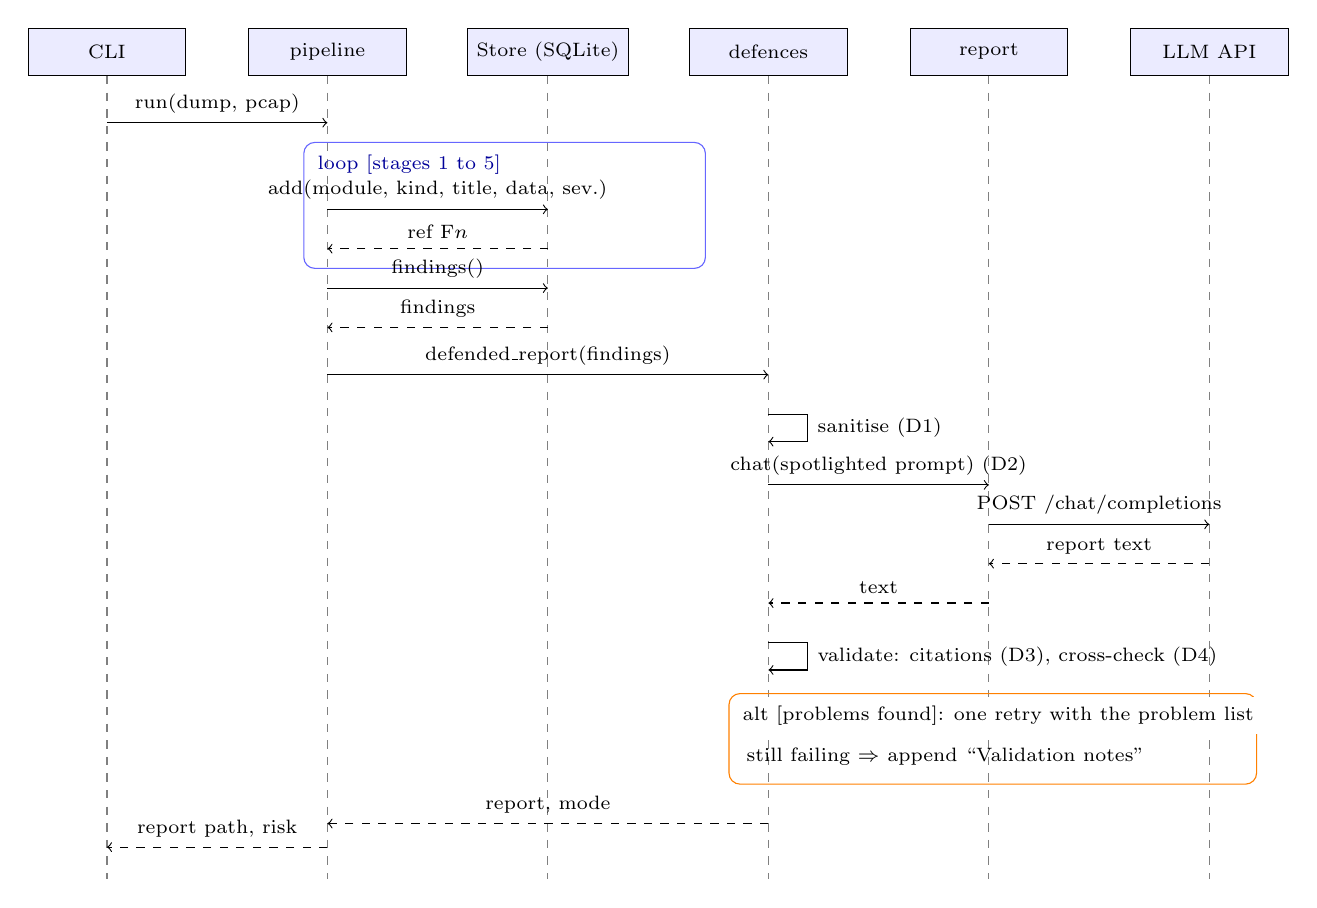
\begin{tikzpicture}[
  actor/.style={draw, fill=blue!8, font=\scriptsize, minimum width=20mm, minimum height=6mm, align=center},
  msg/.style={->, font=\scriptsize},
  ret/.style={->, dashed, font=\scriptsize}]
  \foreach \x/\n/\l in {0/cli/CLI, 2.8/pipe/pipeline, 5.6/store/Store (SQLite), 8.4/def/defences, 11.2/rep/report, 14/groq/LLM API} {
    \node[actor] (\n) at (\x,0) {\l};
    \draw[gray, dashed] (\n.south) -- ++(0,-10.2);
  }
  \def\y{-0.9}
  \draw[msg] (0,-0.9) -- node[above]{run(dump, pcap)} (2.8,-0.9);
  \draw[draw=blue!60, rounded corners] (2.5,-1.15) rectangle (7.6,-2.75);
  \node[font=\scriptsize, anchor=north west, text=blue!60!black] at (2.55,-1.18) {loop [stages 1 to 5]};
  \draw[msg] (2.8,-2.0) -- node[above]{add(module, kind, title, data, sev.)} (5.6,-2.0);
  \draw[ret] (5.6,-2.5) -- node[above]{ref F$n$} (2.8,-2.5);
  \draw[msg] (2.8,-3.0) -- node[above]{findings()} (5.6,-3.0);
  \draw[ret] (5.6,-3.5) -- node[above]{findings} (2.8,-3.5);
  \draw[msg] (2.8,-4.1) -- node[above]{defended\_report(findings)} (8.4,-4.1);
  \draw[msg] (8.4,-4.6) -- ++(0.5,0) -- ++(0,-0.35) node[right, pos=0.5]{sanitise (D1)} -- ++(-0.5,0);
  \draw[msg] (8.4,-5.5) -- node[above]{chat(spotlighted prompt) (D2)} (11.2,-5.5);
  \draw[msg] (11.2,-6.0) -- node[above]{POST /chat/completions} (14,-6.0);
  \draw[ret] (14,-6.5) -- node[above]{report text} (11.2,-6.5);
  \draw[ret] (11.2,-7.0) -- node[above]{text} (8.4,-7.0);
  \draw[msg] (8.4,-7.5) -- ++(0.5,0) -- ++(0,-0.35) node[right, pos=0.5]{validate: citations (D3), cross-check (D4)} -- ++(-0.5,0);
  \draw[draw=orange, rounded corners] (7.9,-8.15) rectangle (14.6,-9.3);
  \node[font=\scriptsize, anchor=north west, fill=white] at (7.95,-8.18) {alt [problems found]: one retry with the problem list};
  \node[font=\scriptsize, anchor=west] at (8.0,-8.95) {still failing $\Rightarrow$ append ``Validation notes''};
  \draw[ret] (8.4,-9.8) -- node[above]{report, mode} (2.8,-9.8);
  \draw[ret] (2.8,-10.1) -- node[above]{report path, risk} (0,-10.1);
\end{tikzpicture}
\caption{UML sequence diagram of an analysis run with the defended LLM report.}
\label{fig:seq}
\end{figure*}

\begin{figure*}[!ht]
\centering
\begin{tikzpicture}[
  cls/.style={draw, rectangle split, rectangle split parts=3, align=left, font=\scriptsize,
              rectangle split part fill={blue!12,white,white}, inner sep=2pt, text width=40mm},
  mod/.style={draw, rectangle split, rectangle split parts=2, align=left, font=\scriptsize,
              rectangle split part fill={green!12,white}, inner sep=2pt, text width=40mm}]
  \node[cls] (store) at (0,0) {\textbf{Store}\nodepart{second}db: sqlite3.Connection\\run\_id: int\\n: int
    \nodepart{third}start\_run(dump, pcap)\\add(module, kind, title, data, severity, source, location): ref\\findings(run\_id): list\\commit(); close()};
  \node[mod] (pipe) at (6,0) {\textbf{$\langle\langle$module$\rangle\rangle$ pipeline}\nodepart{second}run(dump, pcap, binaries, use\_llm, defended)\\record\_crypto(db, path, result, is\_full\_dump)};
  \node[mod] (crypto) at (12,0) {\textbf{$\langle\langle$package$\rangle\rangle$ crypto}\nodepart{second}analyse(path)\\entropy.high\_entropy\_regions()\\identify.identify\_file(); score()\\rsa\_weak.extract\_keys(); assess()};
  \node[cls] (sig) at (12,-3.6) {\textbf{Sig}\nodepart{second}algo, name, pattern\\weight, kind, wide\nodepart{third}(56 instances in signatures.py)};
  \node[mod] (mem) at (0,-3.6) {\textbf{memory / static / credentials / network}\nodepart{second}extract(); suspicious\_processes()\\analyse(); scan(); parse(); weak\_tls()};
  \node[mod] (rep) at (6,-3.6) {\textbf{report / defences}\nodepart{second}risk\_score(); rule\_report(); chat()\\sanitise(); check\_citations()\\cross\_check(); defended\_report()};
  \node[cls] (att) at (6,-7) {\textbf{Attack}\nodepart{second}name, goal, payload\\succeeded(text, findings)\nodepart{third}(6 attacks in redteam.py)\\redteam.run(trials, dry\_run, rescore)};
  \draw[->, dashed] (pipe) -- node[above, font=\scriptsize]{uses} (store);
  \draw[->, dashed] (pipe) -- node[above, font=\scriptsize]{uses} (crypto);
  \draw[->, dashed] (pipe) -- (mem);
  \draw[->, dashed] (pipe) -- (rep);
  \draw[{Diamond[open]}-] (crypto) -- node[right, font=\scriptsize]{1..*} (sig);
  \draw[->, dashed] (att) -- node[right, font=\scriptsize]{evaluates} (rep);
\end{tikzpicture}
\caption{UML class and module diagram (main classes and public functions).}
\label{fig:class}
\end{figure*}

\begin{figure}[!ht]
\centering
\begin{tikzpicture}[node distance=4mm,
  act/.style={draw, rounded corners=6pt, fill=blue!6, font=\scriptsize, align=center, minimum height=5mm, inner sep=2pt},
  dec/.style={draw, diamond, aspect=2.4, fill=yellow!12, font=\scriptsize, align=center, inner sep=0.5pt}]
  \node[circle, fill=black, minimum size=2.5mm, inner sep=0] (st) {};
  \node[act, below=of st] (a) {malfind region (RWX, unbacked)};
  \node[dec, below=of a] (d1) {starts with MZ?};
  \node[act, right=6mm of d1, fill=red!15] (c) {critical};
  \node[dec, below=of d1] (d2) {known JIT process\\or zeroed start?};
  \node[act, right=6mm of d2, fill=blue!12] (l) {low};
  \node[dec, below=of d2] (d3) {same code in\\$\ge$3 processes?};
  \node[act, right=6mm of d3, fill=yellow!25] (m) {medium};
  \node[act, below=of d3, fill=orange!25] (h) {high (unique injection)};
  \draw[->] (st) -- (a); \draw[->] (a) -- (d1);
  \draw[->] (d1) -- node[above, font=\scriptsize]{yes} (c);
  \draw[->] (d1) -- node[left, font=\scriptsize]{no} (d2);
  \draw[->] (d2) -- node[above, font=\scriptsize]{yes} (l);
  \draw[->] (d2) -- node[left, font=\scriptsize]{no} (d3);
  \draw[->] (d3) -- node[above, font=\scriptsize]{yes} (m);
  \draw[->] (d3) -- node[left, font=\scriptsize]{no} (h);
\end{tikzpicture}
\caption{UML activity diagram: grading an injected-code region.}
\label{fig:activity}
\end{figure}
